\documentclass[a4paper,11pt]{article}
\usepackage[ngerman]{babel}
\usepackage[utf8]{inputenc}
\usepackage{amsmath}
\usepackage{hyperref}
\usepackage{graphicx}
\usepackage{listings}

\title{Abgabe 1 für Computergestützte Methoden}
\author{Gruppe 21, 4371147 Maximilian Lietzau, 4166459 Louis Koch)}
\date{02.12.2024}

\begin{document}

\maketitle

\tableofcontents

\newpage

\section{Der zentrale Grenzwertsatz}
Der zentrale Grenzwertsatz (ZGS) ist ein fundamentales Resultat der Wahrscheinlichkeitstheorie, das die Verteilung von Summen unabhängiger, identisch verteilter (i.i.d.) Zufallsvariablen (ZV) beschreibt. Er besagt, dass unter bestimmten Voraussetzungen die Summe einer großen Anzahl solcher ZV annähernd normalverteilt ist, unabhängig von der Verteilung der einzelnen ZV. Dies ist besonders nützlich, da die Normalverteilung gut untersucht und mathematisch handhabbar ist.

\subsection{Aussage}
Sei \( X_1, X_2, \dots, X_n \) eine Folge von i.i.d. ZV mit dem Erwartungswert \( \mu = E(X_i) \) und der Varianz \( \sigma^2 = \text{Var}(X_i) \), wobei \( 0 < \sigma^2 < \infty \) gilt. Dann konvergiert die standardisierte Summe \( Z_n \) dieser ZV für \( n \to \infty \) in Verteilung gegen eine Standardnormalverteilung \footnote{  Der zentrale Grenzwertsatz hat verschiedene Verallgemeinerungen. Eine davon ist der
Lindeberg-Feller-Zentrale-Grenzwertsatz [\cite{Klenke2013}, Seite 328], der schwächere Bedingungen an
die Unabhängigkeit und die identische Verteilung der ZV stellt.}:
\begin{equation}
Z_n = \frac{\sum_{i=1}^{n} X_i - n \mu}{\sigma \sqrt{n}} \xrightarrow{d} N(0, 1).
\label{eq:formel1}
\end{equation}
Das bedeutet, dass für große \( n \) die Summe der ZV näherungsweise normalverteilt ist mit Erwartungswert \( n \mu \) und Varianz \( n \sigma^2 \):
\begin{equation}
\sum_{i=1}^{n} X_i \sim N(n \mu, n \sigma^2).
\label{eq:formel2}
\end{equation}

\subsection{Erklärung der Standardisierung}
Um die Summe der ZV in eine Standardnormalverteilung zu transformieren, subtrahiert man den Erwartungswert \( n \mu \) und teilt durch die Standardabweichung \( \sigma \sqrt{n} \). Dies führt zu der obigen Formel \ref{eq:formel1}. Die Darstellung \ref{eq:formel2} ist für \( n \to \infty \) nicht wohldefiniert.

\subsection{Anwendungen}
Der ZGS wird in vielen Bereichen der Statistik und der Wahrscheinlichkeitstheorie angewendet. Typische Beispiele sind:
\begin{itemize}
    \item Hypothesentests
    \item Sch\"atzungen statistischer Kennzahlen in großen Stichproben
\end{itemize}

\section{Bearbeitung zur Aufgabe 1}

\subsection{Thema Datenverarbeitung}
Zuerst haben wir die CSV-Datei in die Tabellenkalkulation Excel eingespielt. Da die Daten alle zusammen in einer Spalte standen mussten wir diese mit dem Befehl Text in Spalten trennen, sodass wir für jedes Komma eine eigene Spalte erhalten haben. Hierbei mussten wir beachten, dass die Nachkommastellen in der Amerikanischen Schreibweise durch einen Punkt getrennt werden. Dann haben wir die für unsere Gruppe nicht relevanten Datensätze gelöscht. Im nächsten Schritt haben wir nun mit dem Befehl \textit{MAX(J2:J366)} die höchste durchschnittliche Temperatur ermittelt. Diese beträgt für unsere Gruppe 83° Fahrenheit. Für die Datenpunkte 99 und 343 gab es für die maximale durchschnittliche Temperatur keine Werte, an den Tagen davor und danach waren die Werte allerdings signifikant niedriger, sodass es ausgeschlossen ist, dass die Temperatur an diesen Tagen höher war. Mit dem Befehl \textit{UMWANDELN(D369; "F";"C")} Haben wir dann wie in der Aufgabe gefordert die Temperatur in Grad Celsius umgewandelt. Für unsere Gruppe beträgt die maximale durchschnittliche Temperatur 28,33 ° Celsius 

\subsection{Thema Datenhaltung}
\begin{figure}[h]
\centering
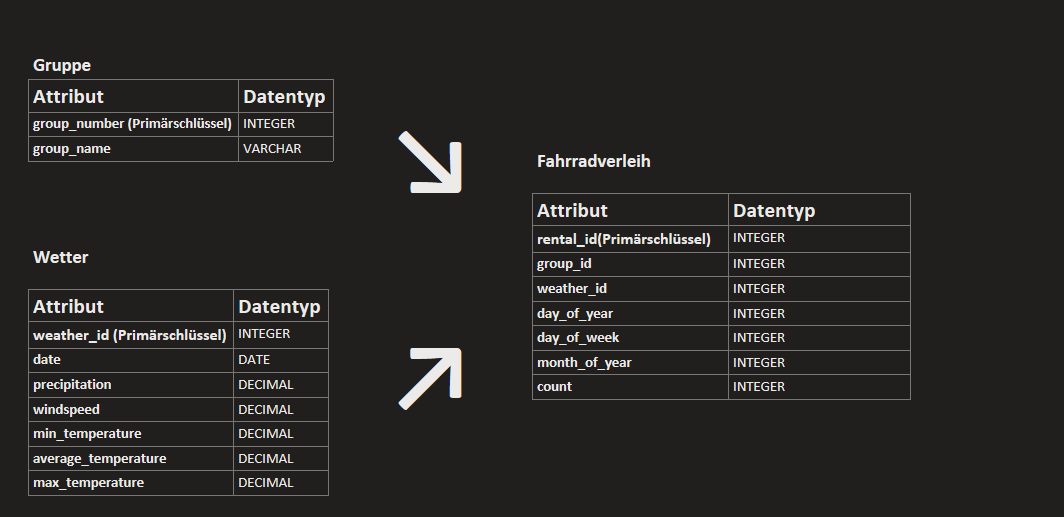
\includegraphics[scale=.5]{Datenbankschema.png}
\caption{Datenbankschema}
\label{fig:meine-grafik}
\end{figure}

 
\subsection{Erstellung Tabellen}
Für die Erstellung der Datenbank haben wir folgende SQL Befehle genutzt: 


\begin{figure}[h]
\centering
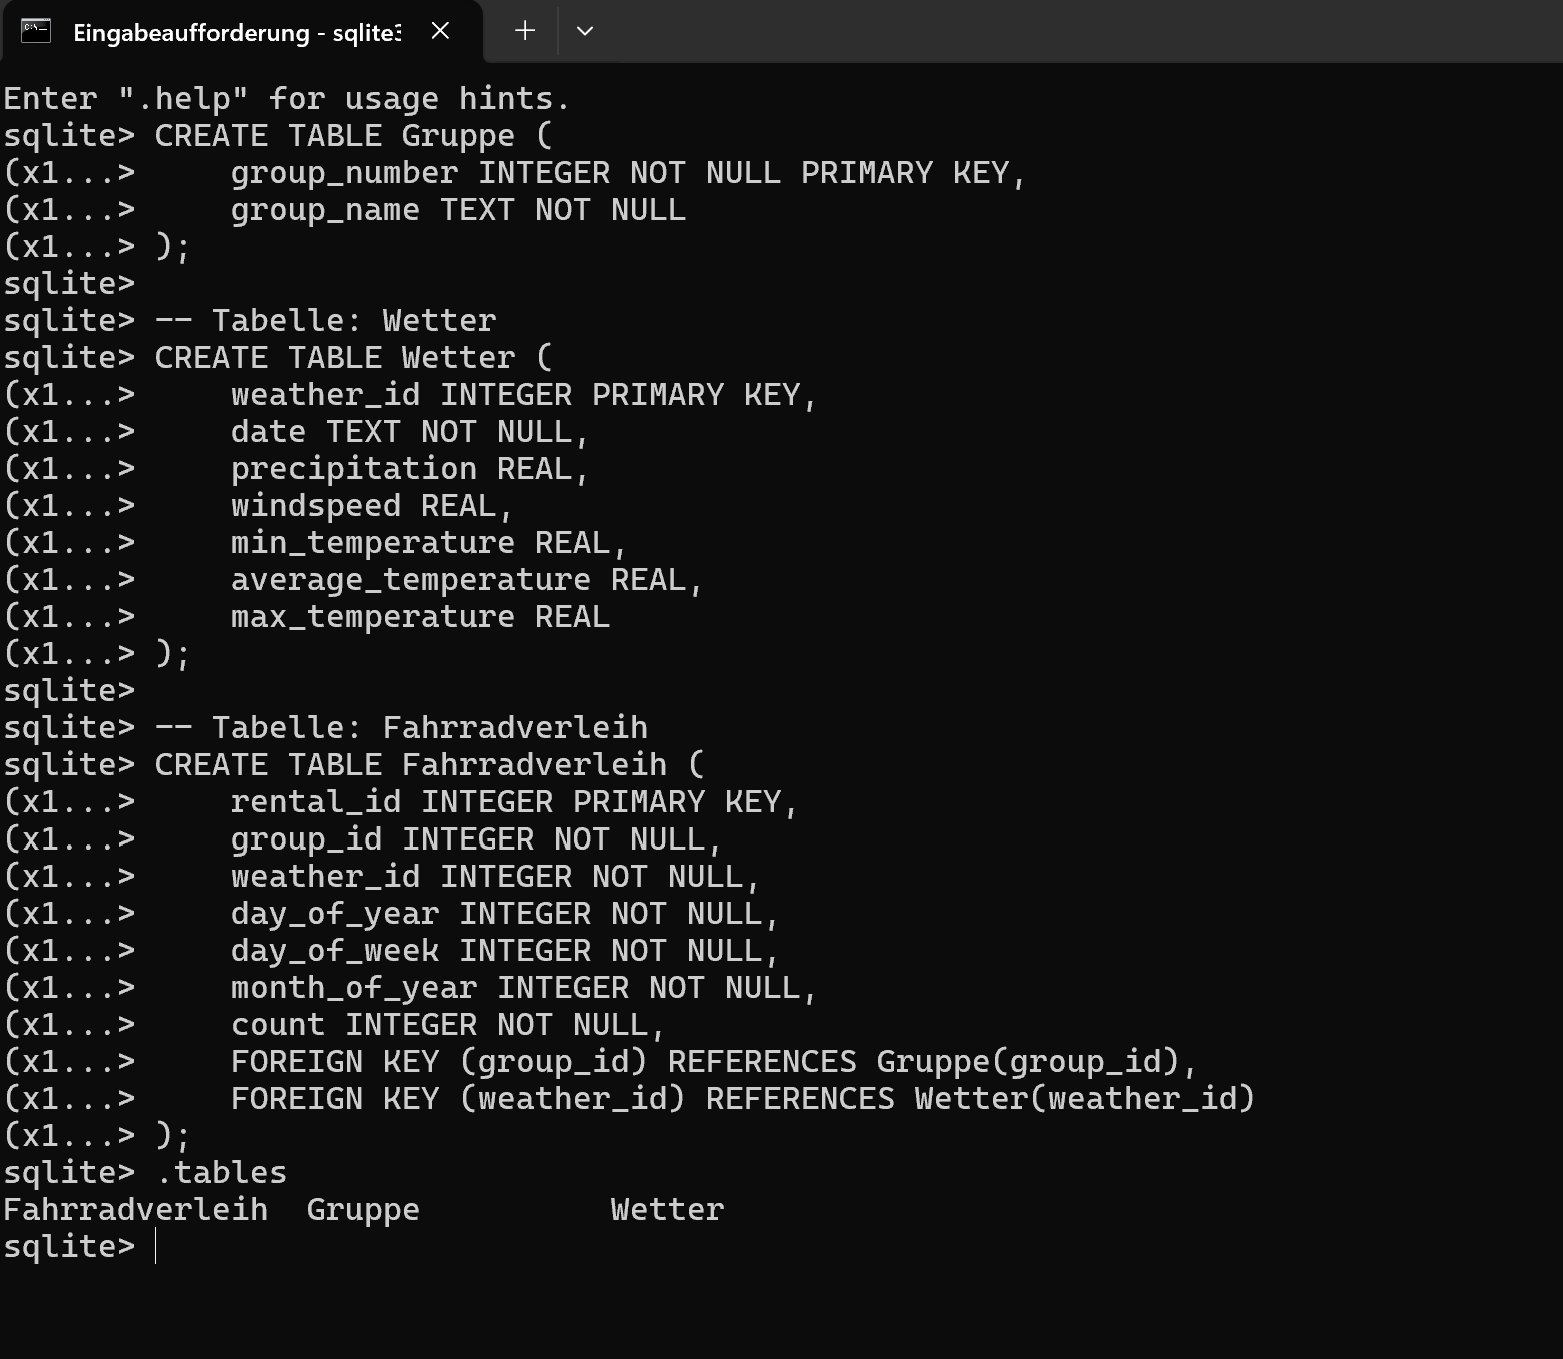
\includegraphics[scale=.5]{Tabellen erstellen.png}
\caption{SQL Befehle zur Erstellung unserer Tabellen}
\label{fig:meine-grafik2}
\end{figure}

\subsection{Import der Daten}
Zur Vorbereitung auf das Importieren der Daten, haben wir die CSV Datei mit Excel geöffnet. In Excel haben wir dann nach ungültigen Werten gesucht. An Tag 99 fehlten beispielsweise die Werte für den Niederschlag und die durchschnittliche Temperatur. Die fehlenden Werte für den Wochentag, Monat und Tag des Jahres können sehr einfach ergänzt werden, da diese immer fortlaufend sind, bzw sich immer wiederholen und daher genau zu bestimmen sind. Für die fehlenden Werte der Durchschnittstemperatur haben wir die niedrigste und die höchste Temperatur des Tages addiert und durch 2 geteilt. Für die fehlenden Werte der niedrigsten und der höchsten Tagestemperatur haben wir dies ähnlich gemacht und ungefähre Werte geschätzt. Außerdem haben wir die Werte der umliegenden Tage in unserer Schätzung berücksichtigt. Es gab zudem auch einige negative Werte, welche entweder keinen Sinn ergeben haben. Es kann beispielsweise nicht -1 Fahrrad vermietet werden und wenn die niedrigste Temperatur positiv ist, kann die höchste nicht negativ sein.
Zur Vereinfachung haben wir nun aus der Excel Tabelle insgesamt 3 Tabellen gemacht, um diese dann in die richtigen Datenbank einspielen zu können. In diesen Tabellen haben wir dann auch die noch fehlenden Primärschlüssel definiert. 
Dann haben wir die Daten mit ",import" in die Datenbanken eingespielt. 

\subsection{Abfrage der höchsten Durchschnittstemperatur}

Für die Abfrage der höchsten Durchschnittstemperatur benutzen wir die Befehle 

\begin{figure}[h]
\centering
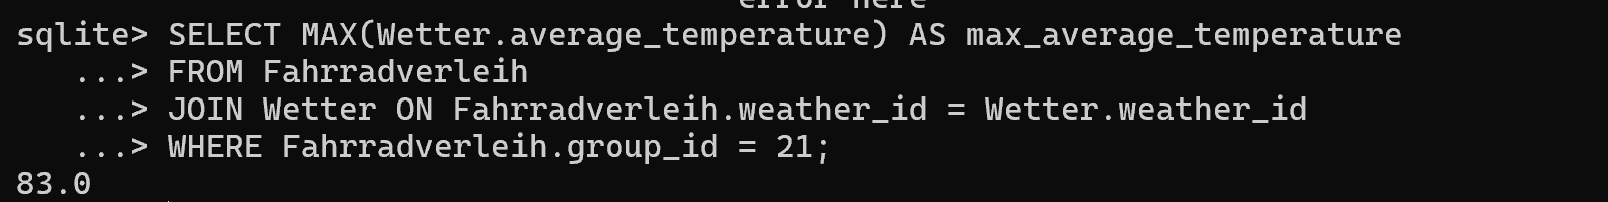
\includegraphics[scale=.5]{Abfrage.png}
\caption{Die Abfrage in Fahrenheit}
\label{fig:meine-grafik3}
\end{figure}

\begin{figure}[h]
\centering
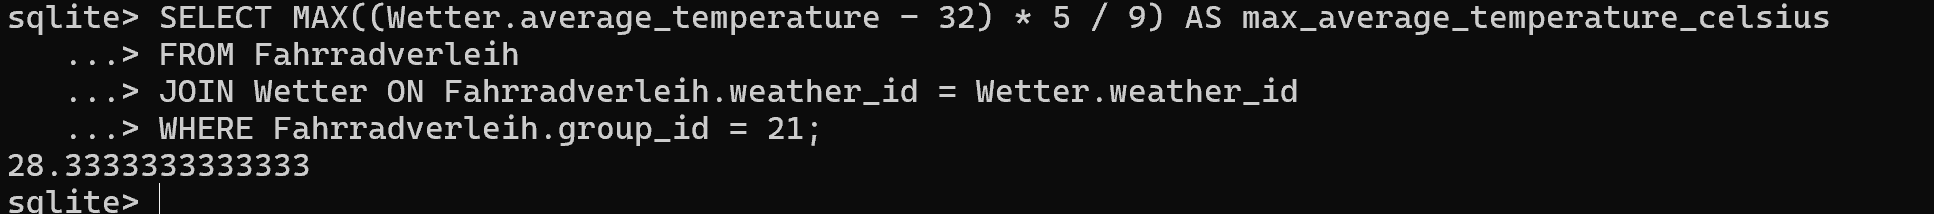
\includegraphics[scale=.4]{Abfrage Celsius.png}
\caption{Die Abfrage umgerechnet in Grad Celsius}
\label{fig:meine-grafik4}
\end{figure}

\begin{thebibliography}{9}
\bibitem{Klenke2013}
Achim Klenke. \textit{Wahrscheinlichkeitstheorie}. Springer, 3. Auflage, 2013.
\end{thebibliography}

\end{document}
